% ------------------------------------
% UNIVERSIDAD DE COSTA RICA
% Facultad de Ingeniería
% Escuela de Ingeniería Eléctrica
% IE0499 - Proyecto Eléctrico
%
% PLANTILLA Y GUÍA DEL TRABAJO ESCRITO
% Versión: v1.0 (marzo 2017)
% ------------------------------------

% Tipo de documento
\documentclass[final]{proyectoelectrico}

% A. PAQUETES Y MACROS ESPECIALES -------
% Paquetes y definiciones que no están incluidos 
% en la clase proyectoelectrico.cls o que son 
% propios del proyecto.
% -----------------------------------------
% OTROS PAQUETES E INSTRUCCIONES ESPECIALES
% -----------------------------------------

% PAQUETES
%%%%%%%%%%

% Para insertar PDFs
\usepackage{pdfpages}

% Para insertar código fuente estilizado
\usepackage{listings}
	\lstset{basicstyle=\ttfamily,
    		breaklines=true,
            numbers=left, 
    		numberstyle=\tiny, 
    		stepnumber=1, 
    		numbersep=6pt
            }

% Para usar múltiples columnas
\usepackage{multicol}

% Para crear árboles conceptuales
\usepackage{forest}

% Para insertar símbolos extraños
\usepackage{marvosym}

% Para insertar texto fútil
\usepackage{lipsum}


% NUEVAS INSTRUCCIONES
%%%%%%%%%%%%%%%%%%%%%%

\newcommand{\EIEx}{\textsc{Escuela \Lightning~ Ingeniería Eléctrica}}

% Definición de algunos símbolos matemáticos
\newcommand{\me}{\mathrm{e}}
\newcommand{\mi}{\mathrm{i}}
\newcommand{\mj}{\mathrm{j}}
\newcommand{\md}{\mathrm{d}}

% Listas con menos espacio entre ítemes (más ajustado)
\newcommand{\ajustado}{\itemsep0pt\parskip0pt\parsep0pt}

% FORMATO PARA EL REGLAMENTO
%%%%%%%%%%%%%%%%%%%%%%%%%%%%

\newcounter{articulo}
\newcommand{\articulo}[2]{
	{
    \stepcounter{articulo}
    \noindent
	\textbf{Artículo \thearticulo} --- \textit{#1}
	\vspace{2mm}\\
	}{
	#2
	\vspace{2mm} \\
	}
}

\newcounter{capitulo}
\newcommand{\capitulo}[1]{
	{
    \stepcounter{capitulo}
    \centering\large\bfseries
    Capítulo \Roman{capitulo}. #1
    \vspace{4mm}\\
    }
}

% Tipografía
\usepackage{libertine}
\usepackage{libertinust1math}
\usepackage[T1]{fontenc}
\renewcommand*{\ttdefault}{cmtt}
% ---------------------------------------

% B. DATOS ------------------------------
% Todos los nombres incluyen dos apellidos,
% acentos y signos de puntuación apropiados.
% Revisar las recomendaciones sobre el título
% y los nombres de los profesores en la guía.

% Título del proyecto
\titulo{Aplicación móvil para el reconocimiento y registro de placas numeradas con aprendizaje automático para el inventario de activos en E.I.E.}

% Autor (nombre y carné)
\autor{Isaac Rojas Hernández}
\carne{B76693}

% Profesor(a) guía
% (Ing.) Nombre Apellido Apellido(, título)
\guia{Ing. Marco Villalta Fallas, M.Sc}

% Profesores lectores 
\lectorA{Ing. Marvin Coto Jimenez, PhD.}
\lectorB{Ing. Harold Moreno Urbina, M.Sc}

% Fecha de entrega del trabajo escrito
\mes{1}		% Número del mes
\ano{2023}	% Formato AAAA
% ---------------------------------------

% C. CONTENIDOS -------------------------

%%%%%%%%%%%%%%%%%%%
\begin{document}
%%%%%%%%%%%%%%%%%%%

\frontmatter

% 1. PORTADA
\portada

% 2. HOJA DE APROBACIÓN
\iffinal
\aprobacion
\fi

% 3. RESUMEN (EN ESPAÑOL E INGLÉS)
% EL RESUMEN
% ----------

\begin{resumen}{OCR, Red Neuronal, Android, Aplicación, Inventario, Automatización}

La automatización de tareas es una forma básica de simplificación del trabajo, así como también es una forma de optimizar diferentes procesos dentro de un entorno. Ahorrar tiempo y facilitar las tareas a las personas es un reto moderno conforme se implementan más tecnologías a la vida cotidiana de las personas. En este proyecto se toma este concepto para poder desarrollar una forma de automatizar la escritura y almacenamiento de los datos de los activos presentes en la Escuela de Ingeniería Eléctrica. Esto se logra por medio del uso de una red neuronal entrenada para OCR y una aplicación para teléfonos móviles Android.

\end{resumen}
% EL RESUMEN EN INGLÉS
% --------------------

\begin{theabstract}{Mobile inventory app for registration of the assests of the E.I.E with Neural Network}{OCR, Neural Network, Android, App, Inventory, Automatization}

The automatization of tasks is a basic form to simplify work, not only that, but it's also a way to optimize processes in different environments. Saving time and facilitating completion of workload is one of the modern challenges we have to overcome if we want to adapt as new technologies get implemented within daily basis. In this project, this concept is taken as a base to develop a way of automatization for inventory collection within our Electrical Engineering School. To solve this problem, a neural network is implemented and trained to do OCR with an Android app that will act as the front-end to wrap up the network. 
\end{theabstract}

% El entorno 'theabstract' tiene el formato \begin{theabstract}{A} ...B... \end{theabstract} donde A es el título del proyecto traducido de inglés a español y B es el contenido, en inglés, del resumen. Se recomienda buscar ayuda calificada para la elaboración y/o revisión de este resumen.

% 4. RECONOCIMIENTOS
\iffinal
% LOS RECONOCIMIENTOS
% -------------------

% Aquí se escribe la dedicatoria del proyecto y los agradecimientos. El entorno 'reconocimiento' tiene la estructura \begin{reconocimiento}{Dedicatoria} Agradecimientos \end{reconocimiento}

\begin{reconocimiento}{Dedicado a mis papás, a mi hermanito menor, a mi Tío Naty y a todas las peronas que fueron luz durante mis años universitarios.}

En primer lugar quiero agradecer a mi tutor Marco, por aceptar trabajar conmigo como guía en este proyecto, a la Escuela de Ingeniería Eléctrica por haber sido mi hogar vocacional durante todos estos años y a todos los profesores que me instruyeron dentro de mi vida académica. Así mismo, quiero agradecerle a mis papás por apoyarme desde el día uno, por ayudarme a aprovechar la oportunidad de la educación superior y por estar conmigo aún cuando yo no tenía fuerzas para seguir. A mi tío Naty por ser uno de los mayores promotores en mi vida académica, por estar dispuesto a siempre darme un consejo, por nunca juzgarme y por ser una de las personas que más admiro. A mi hermano menor, porque gracias a él me motivo a ser mejor todos los días, para llegar a ser un profesional que admire, que busque y que pueda consentirlo en todo siempre. Por último quiero agradecerle a todas las personas que llamo o he llamado en algún momento mis amigos, porque siempre los llevo en mi corazón y sé que en algún momento de mi vida universitaria fueron el pequeño impulso que necesité para seguir, además agradezco a todos los que se encuentran hoy conmigo viendo como finalizo esta etapa y empiezo la nueva, gracias por estar aquí y gracias por enseñarme cosas nuevas todos los días.

\end{reconocimiento}
\fi

% 5. TABLAS DE CONTENIDO, FIGURAS Y TABLAS
\tableofcontents
\newpage
\listoffigures
\newpage
\listoftables

% 6. NOMENCLATURA
% LA NOMENCLATURA
% ---------------

% La nomenclatura se realiza con el paquete 'nomencl'. Para ingresar un nuevo elemento, se debe usar el comando \nomenclature{símbolo}{definición}, ya sea en este archivo nomenclatura.tex (más fácil para encontrar y editar), o en cualquier parte del documento (probablemente cuando se introduce una nueva variable o constante). Para más opciones del paquete, favor referirse a su documentación (https://www.ctan.org/pkg/nomencl). También hay una buena guía de uso en https://www.sharelatex.com/learn/Nomenclatures.

% Formato recomendado
% -------------------

% Variable o constante matemática
% \nomenclature{$V$}{Tensión eléctrica}

% Acrónimo
% \nomenclature{TBH}{Para ser honesto (del inglés \textit{To Be Honest})}

% Si únicamente existen acrónimos del inglés, se puede omitir la frase 'del inglés'. La definición no tiene punto al final.

\nomenclature{OCR}{Reconocimiento óptico de caracteres (del inglés \textit{Optical Character Recognition })}
\nomenclature{IEEE}{Instituto de Ingenieros Eléctricos y Electrónicos (del inglés \textit{Institute of Electrical and Electronics Engineers})}
\nomenclature{EIE}{Escuela de Ingeniería Eléctrica de la Universidad de Costa Rica}
\nomenclature{SGBD}{Sistemas de gestión de bases de datos.}
\nomenclature{API}{Interfaz de programación de aplicaciones (del inglés \textit{Application Programming Interface}) }
\nomenclature{BD}{Base de datos}


\printnomenclature

\mainmatter

% 7. CAPÍTULOS
% ----------------------
  \chapter{Introducción}
% ----------------------
\label{C:introduccion}
Dentro de la Universidad de Costa Rica, cada una de las escuelas de carreras tienen el deber de mantener año tras año un inventario de todos los activos que poseen. Con la cantidad tan grande de estudiantes que se aloja en ella, los materiales requeridos para poder dar una educación de calidad es igual o inclusive mayor, por lo que un inventario puede llegar a tomar bastante tiempo y requerir de múltiples personas que lo hagan. Automatizar el proceso de inventariado en algún nivel conllevaría a una reducción significativa de la carga que esto conlleva.
\par
Una de las herramientas que actualmente se utiliza para poder automatizar muchas tareas en el campo laboral y cotidiano, es la inteligencia artificial, más específicamente las redes neuronales. Al tener la capacidad de resolver problemas, realizar tareas, hacer cálculos entre otras aplicaciones, así como la capacidad de aprender constantemente conforme obtienen un buen o un mal resultado, resultan una herramienta muy útil para automatizar procesos.
\par
En el presente trabajo, se busca realizar una aplicación directa de una red neuronal, que logre recibir imágenes tomadas de las placas de los activos, para extraer el número en ellas y registrarla en conjunto con otros datos que los describan. Además se pretende encapsular la aplicación por medio de una aplicación para dispositivos Android, que permita el fácil uso del escáner de placas.

\section{Alcances}
Para poder tener un desarrollo debido del proyecto, primeramente se investigó sobre las redes neuronales: como aplicarlas, como crearlas y como entrenarlas. Por los requerimientos técnicos que conllevan implementar una red neuronal local, se investigó sobre servicios que implementen redes neuronal en la nube y permitan realizar modificaciones en la misma para diferentes aplicaciones requeridas, en este caso se buscó que fuese posible realizar reconocimiento óptico de caracteres con ellas. 
\par
Se estudió también la metodología para el desarrollo de una aplicación móvil sencilla para Android, por medio del lenguaje de programación Python. Así mismo, se estudió las bibliotecas de visión por computador para poder hacer uso de las cámaras de los móviles, módulos de conexión a servidores y por último como almacenar en bases de datos por medio de código para los datos de los activos.
\par
Finalmente con todos estos conceptos estudiados se entrenó la red neuronal, al mismo tiempo que se desarrolló una interfaz gráfica para Android, que tome las capturas, envíe a la red para su lectura y permita almacenar los datos en un servidor MySQL.

\section{Justificación}
El trabajo de inventariado puede conllevar mucho esfuerzo y tiempo que, cualquier tipo de facilitación sería de gran ayuda. 
\par
La Escuela de Ingeniería Eléctrica al tener una población significativa de estudiantes y un edificio grande, puede tener un proceso de inventario mucho más extenso que otras escuelas, además de que el proceso se realiza año con año.
\par
Bajo estos parámetros se contextualiza el presente proyecto, buscando realizar una herramienta que permita al área administrativa de la EIE una fácil realización de su inventario año tras año. 

\section{Objetivos}
\subsection{Objetivo general}
\begin{itemize}
    \item Desarrollar una aplicación móvil con algoritmos automáticos que facilite el inventario realizado en la escuela.
\end{itemize}
\subsection{Objetivos específicos}
\begin{itemize}
    \item Investigar sobre el aprendizaje automático/redes neuronales, procesamiento de imágenes y aplicaciones móviles en Android.
    \item Diseñar un algoritmo para la detección de números a partir de imágenes correspondientes a placas de activos.
    \item Crear una aplicación móvil que implemente el algoritmo diseñado para el registro de los activos con sus placas.
    \item Crear una interfaz amigable y sencilla de usar para el usuario final, para la aplicación. 
    \item Validar el funcionamiento correcto de la aplicación móvil junto con el algoritmo implementado.
\end{itemize}

\section{Metodología}
Con el fin de poder desarrollar el presente proyecto se seguirán los siguientes pasos:
\begin{itemize}
    \item Investigar sobre las redes neuronales y como usarlas para OCR.
    \item Buscar una alternativa basada en web, que permita usar una red neuronal dentro de ella y hacerle envío de archivos para su procesamiento.
    \item Entrenar la red neuronal para pueda detectar los números de las placas de los activos de la escuela.
    \item Aprender a enviar los archivos por medio de un script de python, así como extraer los resultados de los mismos.
    \item Investigar sobre los módulos que permiten crear aplicaciones Android con Python.
    \item Diseñar una interfaz gráfica para Android que integre el algoritmo de la red neuronal
    \item Investigar sobre el almacenamiento de datos por medio de bases de datos.
    \item Hacer que la aplicación almacene los datos coleccionados en una base de datos.
    
\end{itemize}

\section{Cronograma}
\begin{figure}[H]
\centering
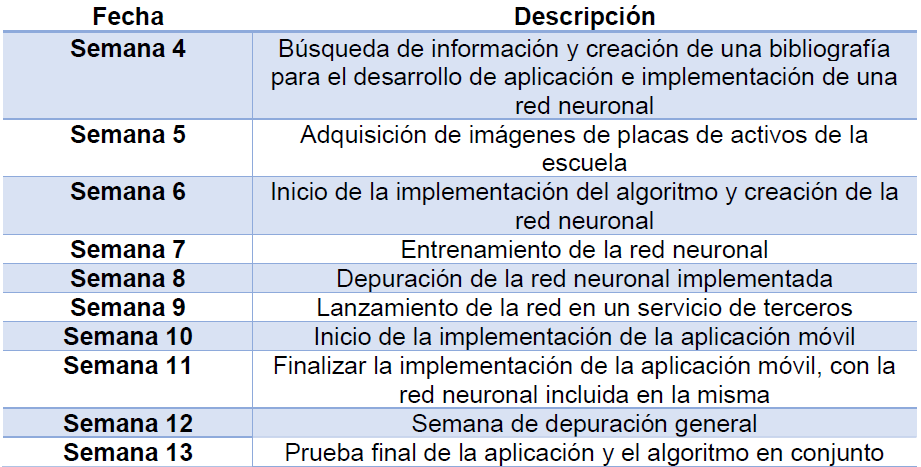
\includegraphics[width=\textwidth]{imagenes/Cronograma.png} 
\caption{Cronograma del proyecto eléctrico}
\label{F:crono}
\end{figure}

% ----------------------
  \chapter{Marco Teórico} 
% ----------------------
\label{C:antecedentes}
Durante el presente capítulo se desarrollará un repaso sobre los principales conceptos relacionados al proyecto, con el fin de poder consolidar una base teórica esencial para entender el mismo.
\section{Redes Neuronales}
\begin{figure}[H]
    \centering
    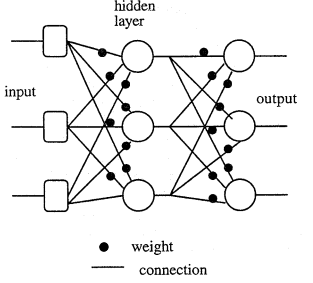
\includegraphics[width=0.5\textwidth]{imagenes/marco teorico/modelo_red.png}
    \caption{Modelo de una red neuronal \cite{nallasamy}}
    \label{neural_model}
\end{figure}
\par
En la figura \ref{neural_model}, se puede ver una representación gráfica para un modelo de una red neuronal, en este caso la aplicada por los autores en \cite{nallasamy}.
\subsection{Generalidades}
\par
Las redes neuronales como la mostrada anteriormente son una representación computacional del cerebro humano, que intenta dar funcionamiento correcto a la inteligencia artificial. La idea detrás de su creación fue poder crear un algoritmo que funcione como lo haría el cerebro humano, debido a que es la computadora más potente conocida.
\par
Al intentar asimilarse al cerebro humano también copian mecanismos utilizados por el mismo, por ejemplo aprenden de la experiencia, es decir a partir de resultados generados, reciben retroalimentación y así afinan los resultados que puedan dar a futuro \cite{olabe_2008}. Inicialmente el programador debe dar a la red una lista de entradas y una de salidas esperadas dependiendo de la entrada, luego la red deberá entrenarse para poder generar resultados que sigan el patrón de los datos iniciales.
\par
La estructura de una red neuronal artificial conlleva los mismos elementos para cualquier aplicación. Cuenta con diferentes entradas que se combinan usualmente sumadas. Luego las entradas pasan por una o varias neuronas (dependiendo de la arquitectura de la red), las cuales se llaman capas ocultas, puesto que contienen una función de transferencia que procesa los datos para luego alimentar cada una de las diferentes salidas \cite{olabe_2008}.
\par
El elemento más importante de una red neuronal, es la neurona, que en programación se puede ver como un nodo de una estructura abstracta, que genera resultados. Cada entrada se conecta a la neurona por medio de un peso, el cual representa la importancia de esta entrada y luego la neurona toma las entradas multiplicadas por su peso y sumadas, para procesarlas por medio de la función de transferencia generada del proceso de entrenamiento \cite{olabe_2008}.

\subsection{Entrenamiento de la red neuronal}
Cómo se mencionó en la sección anterior, una de las características determinantes de una red neuronal es la capacidad de aprendizaje, por lo que es normal que al inicio los resultados obtenidos con ella no sean los deseados. Para arreglar este problema no se puede utilizar la red de forma inmediata, sino que debe llevar un proceso de entrenamiento, para que a la hora de utilizarla, los resultados obtenidos de las entradas dadas sean correcto o muy aproximados.
\par
El proceso de entrenamiento realiza un ajusto en los pesos que posee cada entrada conforme recibe retroalimentación de las salidas generadas. Esto se logra aplicando diferentes entradas de forma secuencial para una obtención de salidas, que luego se verifican, para asegurar que se ajusten los pesos correctamente conforme se introducen datos \cite{olabe_2008}. Existen dos tipos de entrenamientos: supervisado y no supervisado.
\subsubsection{Entrenamiento supervisado}
El programador deberá dar a los datos de entrada provistos una salida emparejada para que la red pueda comparar y ajustar los pesos. Usualmente se ajusta por medio de un cálculo de porcentaje de error, el cual debe ir disminuyendo hasta ser un valor pequeño, que pueda considerar el resultado correcto \cite{olabe_2008}.
\subsubsection{Entrenamiento no supervisado}
En el caso del entrenamiento no supervisado, no se le provee a la red un set de datos de salida deseados, por lo que no hay comparación ni cálculo del error cometido a la hora de procesar los datos. La forma de ajuste de los pesos de cada entrada se da por medio de una comparación interna de las salidas producidas, para que formen un conjunto de datos consistente \cite{olabe_2008}. 
\subsection{Creación de una red neuronal}
Las redes neuronales pueden ser creadas o aplicadas de diferentes formas. La más compleja siendo la creación directa de la red por medio de programación haciendo uso de diferentes librerías como pueden ser: TensorFlow, Microsoft Cognitive Toolkit, PyTorch, Keras, Theano, entre otras. 
\par
El proceso de creación de una red conlleva no solamente el tiempo para poder implementarla por medio de la librería, sino que también el tiempo de entrenamiento para poder finalmente utilizarla. Es importante hacer notar que usualmente el poder computacional necesario para llevar acabo esto es bastante significativo, por lo que no es siempre conveniente.
\par
La otra forma de creación de una red neuronal, está dada por medio del uso de servicios de redes neuronales que están basadas en la nube. Usualmente son provistas por terceros y permiten modificar diferentes aspectos del modelo dependiendo de la aplicación que se quiera utilizar. Es necesario llevar acabo el ajuste de la red, así como el proceso de entrenamiento para que se pueda utilizar. Algunos de los provedores de este tipo de redes más conocidos son: Nanonets, Edge Impulse, Rossum, DarwinAI y muchas otras más.

\section{OCR}
\subsection{Generalidades}
El reconocimiento óptico de caracteres, conocido por sus siglas en inglés OCR (Optical character recognition) es el proceso de análisis y conversión de letras o caracteres de algun medio u objeto a un caracter ASCII que una computadora pueda reconocer \cite{nallasamy}.
\par
El OCR es usado por muchas aplicaciones, de las cuales se incluye la transformación de cualquier cosa humanamente legible a una representación manipulable por una computadora. El proceso permite escanear de manera óptica, por medio de una entrada de video, los caracteres que se desean procesar por la computadora. La intención del proceso de OCR es permitir a las computadoras procesar automáticamente y sin intervención humana fracciones de texto e inclusive objetos que necesiten ser procesados \cite{Shah2009}.
\par
Los sistemas que implementan OCR, se componen de tres partes principales: Una cámara, software de procesamiento de OCR y una interfaz de salida. El reconocimiento de los caracteres usualmente está procesado por inteligencia artificial (usualmente una red neuronal) que conforme procesa datos nuevos aprende a reconocerlos de mejor manera \cite{Shah2009}. La idea de implementar OCR en los sistemas es evitar el error humano, aumentar la capacidad y tiempo de procesamiento además de permitir un mejor rendimiento a la hora de leer y escribir a archivos. 

\subsection{Implementación}
La implementación del OCR por medio de software se logra con diferentes librerías que combinan la visión por computador y la inteligencia artificial para el procesamiento de las imágenes. En trabajos como los vistos en \cite{nallasamy} y \cite{Shah2009} es posible apreciar como se creó un algoritmo que procese las imágenes a partir de una red neuronal. El algoritmo también debe contemplar el pre-procesamiento de las imagenes para que sean más fácilmente leídas por la red que las procesará después.
\par
Hay múltiples librerías para la implementación de OCR para diferentes lenguajes de programación, inclusive Tesseract, el cual es una librería de redes neuronales, incluye funciones que permiten la implementación de OCR.

\section{Python}
Python es un lenguaje de programación interpretado, es decir un programa intermediario entre la computadora y el usuario (llamado interprete) lee el código y lo ejecuta línea por línea. Es un lenguaje de alto nivel, que al ser creado se pensó especialmente para desarrollo rápido, sencillo, pero aún así poderoso funcional \cite{van1995python}.
\par
Python utiliza sintaxis de escritura sencillo, pensado para la fácil lectura que reduce el costo de la corrección de errores y el fácil entendimiento a la hora de leer el código \cite{van1995python}. Lo que en lenguajes de programación compilados puede tomar varias líneas de código, en Python se reduce de forma significativa. El ejemplo más básico se da a la hora de hacer un programa que imprima "Hola Mundo" en la consola de comandos, como se muestra a continuación:

\begin{lstlisting}[language=Java,frame=single,caption=Código del Hola Mundo en Java, inputencoding=latin1]
public class HolaMundo {

	public static void main(String[] args) {		
		System.out.println("Hola Mundo");
	}

}
\end{lstlisting}
\begin{lstlisting}[language=Python,frame=single,caption=Código del Hola Mundo en Python, inputencoding=latin1]
print("Hola Mundo")
\end{lstlisting}

\par
Es posible notar de los códigos anteriores que la diferencia entre la cantidad de lineas de código en Java es muy superior a la de Python, permitiendo escribir códigos más compactos y más sencillos de leer también. Esto ha hecho que Python sea un lenguaje de programación bastante popular a nivel no-comercial, permitiendo también que se expandan los proyectos que apoyan la creación de librerías para desarrollo en él.


\subsection{Librerías}
\par
Las librerías son un complemento fundamental de la programación en Python, ya que permiten importar a un código funciones previamente escritas que realizan algún algoritmo requerido a la hora de programar \cite{van1995python}.
\par
Con ellas es posible crear códigos para diferentes áreas de aplicación, como por ejemplo el análisis de datos, inteligencia artificial, desarrollo web, ciencias de datos, big data, machine learning e inclusive desarrollo de juegos. La versatilidad que proveen las librerías en conjunto con la facilidad de programación en el lenguaje Python, hacen de la experiencia de desarrollo amigable para cualquier nivel de experiencia que se tenga.

\section{Bases de datos}
Una base de datos es una forma de organizar información o datos con algún tipo de estructura que se almacenan de forma electrónica en un sistema informático. Es decir una base de datos es un conjunto estructurado de datos que representa entidades y sus interrelaciones \cite{camps_paré_2005}.
\par
Para poder controlar las bases de datos, es necesario un gestor que permita hacer un manejo correcto de las mismas. Para ello existen los sistemas de gestión de bases de datos (SGBD). Su principal función es permitir que se hagan consultas no predefinidas y complejas, es decir que la combinación de datos que se quiere extraer de una base de datos no esté predefinida en el programa que la gestiona para que sea una búsqueda válida. Además gestiona las conexiones que se ralizan a la base, por lo que debe permitir y la conexión de varios usuarios a ella \cite{camps_paré_2005}.
\par
Las consultas a la base de datos se realizan por medio de lenguaje escrito (sintaxis) equivalente a un lenguaje de programación, pero específico del tipo de base de datos y el sistema debe interpretar el tipo de acción que se desea realizar. En la figura \ref{BDflux} se puede apreciar el flujo de las consultas a una base de datos. 
\begin{figure}[H]
    \centering
    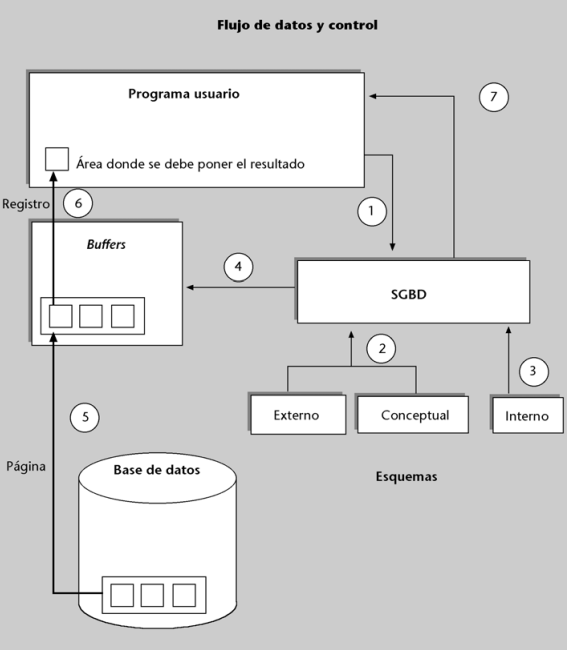
\includegraphics[width=0.4\textwidth]{imagenes/marco teorico/flujo_BD.png}
    \caption{Flujo de una consulta a una base de datos \cite{camps_paré_2005}.}
    \label{BDflux}
\end{figure}
\par
Las consultas inician de forma que se hace una llamada del programa que contacta con la base de datos al SGDB, donde se envía la operación de la consulta que se desea hacer (punto 1). El SGDB verifica que la sintaxis esté correcta y que la conexión esté autorizada a acceder (punto 2) \cite{camps_paré_2005}. 
\par
En caso de que todo esté correcto se debe asegurar que tipo de respuesta requiere la solicitud y cuál aproximación se va a tomar para responderla (punto 3). Luego se revisa si los datos se encuentran cargados en memoria por alguna solicitud previa (punto 4) y caso contrario deberá buscarla en el disco, con ayuda del sistema operativo donde se almacena la BD y cargarla al buffer (punto 5, solo en caso de que no se encuentre previamente cargada)\cite{camps_paré_2005}.
\par
El SGDB realiza operaciones necesarias para poder transportar los datos al área donde se encuentra el programa de la forma más eficiente posible (punto 6). Finalmente el SGDB retorna al programa y devuelve el control al mismo para que haga lo necesario con lo extraído de la base de datos (punto 7) \cite{camps_paré_2005}. 
\par
Con lo mencionado anteriormente es posible comprender el proceso de solicitudes a bases de datos, entiendo así el funcionamiento que se tiene detrás de muchas aplicaciones que contienen datos almacenados en bases de datos.


\subsection{Modelos de bases de datos}
\par
Las bases de datos no se presentan únicamente en un tipo de modelo, sino que a través de los años se han implementado diferentes formas de almacenar los datos dentro de una base de datos y estas se les llaman \textit{modelos de bases de datos}. Se explicará tres de los modelos que se presentan en bases de datos por su relevancia histórica o por su uso popular, siendo estas: jerárquicas, red y relacional, como se observa en la figura \ref{BDmodels}.
\begin{figure}[H]
    \centering
    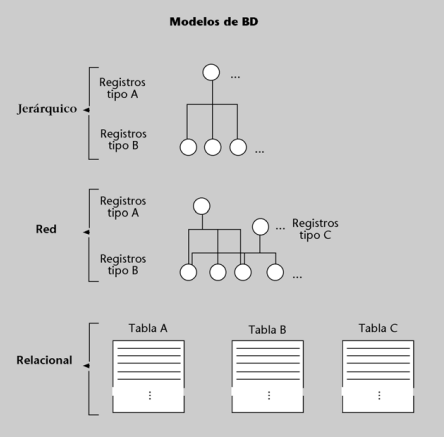
\includegraphics[width=0.5\textwidth]{imagenes/diseño/modelodb.png}
    \caption{Modelos de bases de datos \cite{camps_paré_2005}.}
    \label{BDmodels}
\end{figure}

\subsubsection{Modelo jerárquico}
\par
Fue el primer modelo de BD, surgió a principios de los sesenta. Se estructura está dada como una estructura abstracta de datos de tipo árbol, por lo que los datos están conectados por medio de nodos, que separan los niveles. Es el primer modelo mostrados en la figura \ref{BDmodels} \cite{camps_paré_2005}.

\subsubsection{Modelo de Red}
\par
La estructura de los modelos de red se asemejan a los jerárquicos, con la diferencia de que un registro puede no necesariamente ser hijo de un tipo de registro. Dando una mayor libertad a la organización de datos y su forma de almacenarlos dentro de la BD \cite{camps_paré_2005}, como se presenta en el segundo modelo de la figura \ref{BDmodels}.

\subsubsection{Modelo relacional}
\par
El tercer modelo de la figura \ref{BDmodels} es el relacional, el cual se diferencia mucho de los otros dos modelos presentados anteriormente, esto debido a que está basado en el concepto matemático de relación. Su principal elemento es la tabla, la cual es la causa del nombre que se le asigna. La tabla consta de filas y columnas, donde cada columna usualmente presente un atributo y cada fila es un registro único diferente del resto (aunque no necesariamente con diferentes columnas, a excepción de la característica principal, que es diferenciante). Es una forma intuitiva y sencilla de almacenar datos, ya que a nivel lógico tiene mucho sentido almacenarlos de esta forma, además permite la facilidad de tener más de una tabla donde puede o no alguna de sus filas tener relación con alguna fila y/o columna de otra \cite{camps_paré_2005}.


% --------------------
  \chapter{Diseño}
% --------------------
\label{C:desarrollo}

En la presente sección se desarrolló el diseño la aplicación y los componentes necesarios para que funcione de forma adecuada. Es necesario establecer que para poder diseñar la aplicación se distribuyó las funciones de la misma por medio de distintos componentes. Asegurando así que se tenga pruebas de que cada componente tiene un funcionamiento correcto por separado como en conjunto. En la figura (\ref{appdiagram}), se puede ver como se distribuyó el diseño de la aplicación.
\begin{figure}[H]
    \centering
    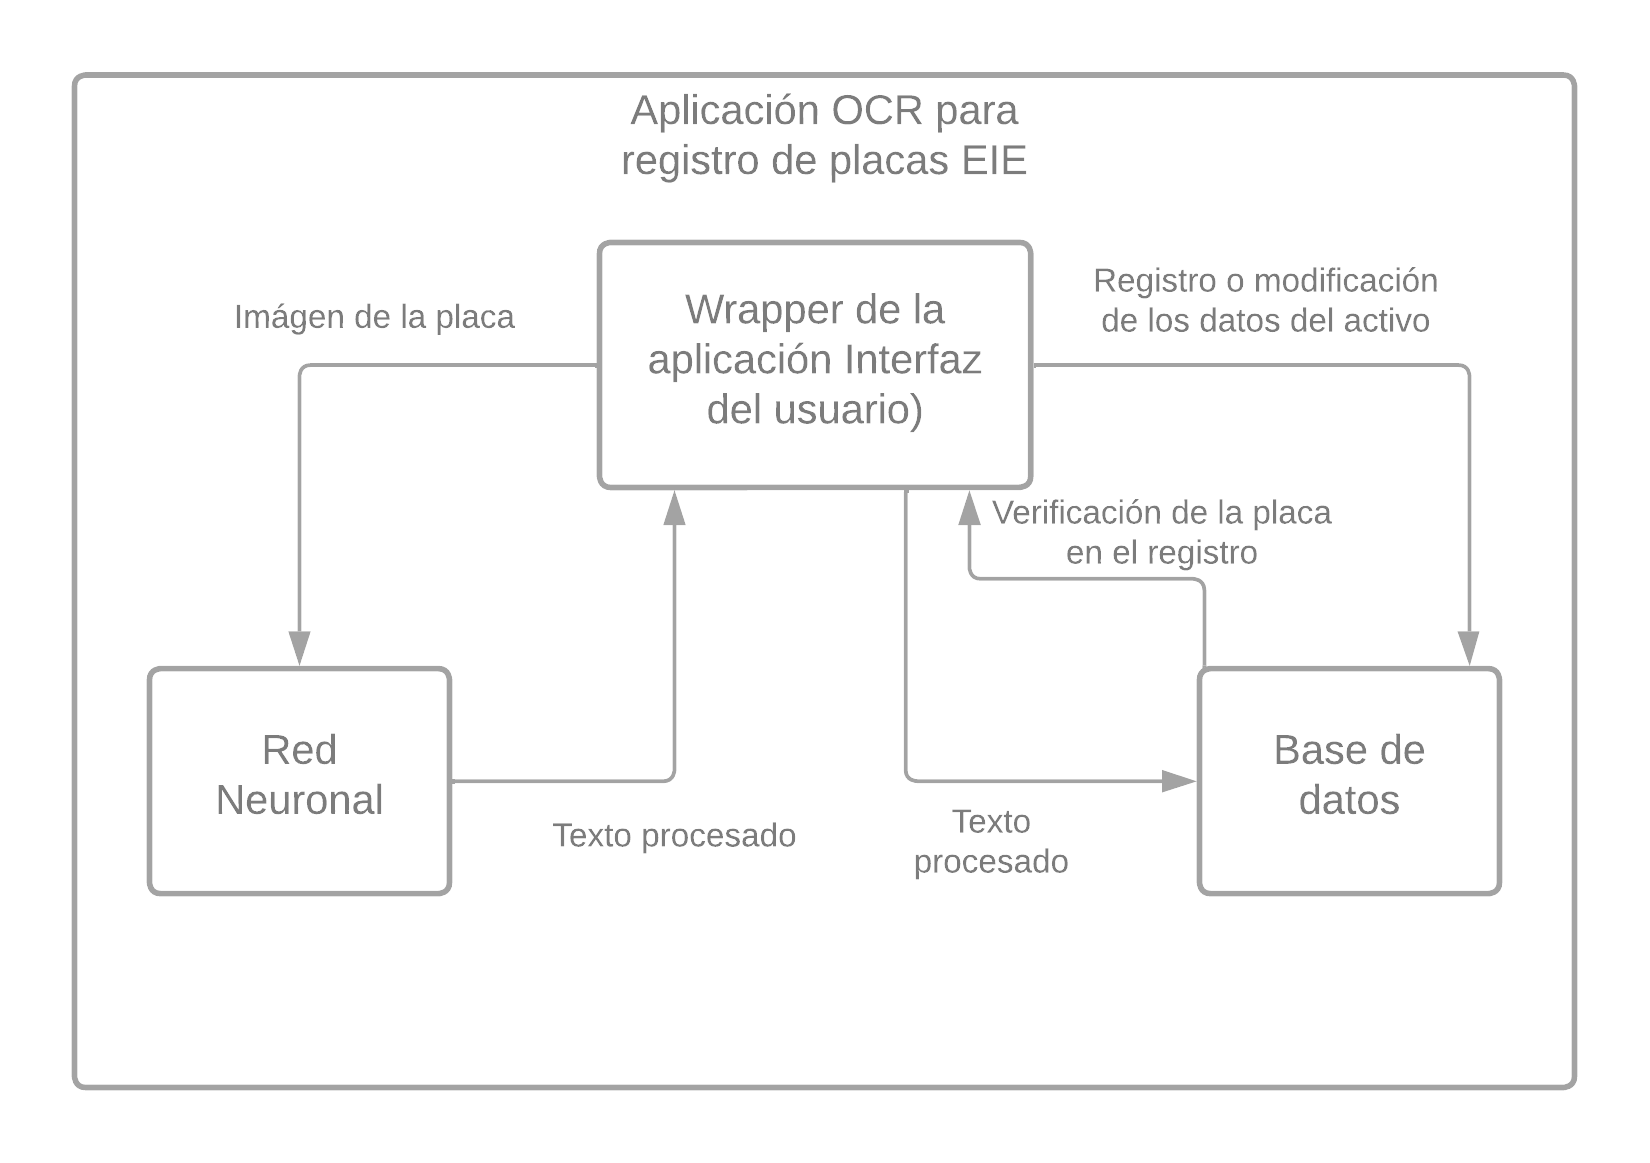
\includegraphics[width=0.7\textwidth]{imagenes/diseño/diagrama_del_programa.png}
    \caption{Diagrama del funcionamiento de la aplicación (creación propia)}
    \label{appdiagram}
\end{figure}
\par
Se creó tres componentes principales para la aplicación, donde el principal sería el wrapper o la interfaz del usuario, la red neuronal y la base de datos. Estos se encuentran conectados entre sí por medio del wrapper, que no solamente permite las entradas y las salidas con los usuarios, sino que también corre las funciones para acceder a cada uno de los componentes.

\section{Red neuronal}
Debido a la complejidad y cantidad de recursos que puede requerir crear una red neuronal completamente de cero, se optó por utilizar una red neuronal pre-fabricada, a la cual se le modificó diferentes parámetros para procesar específicamente imágenes y que realizaran un análisis de OCR. 
\par
El servicio utilizado para este proyecto fue el de Nanonets, debido a que las redes neuronales que ofrecen permiten nativamente adaptarlas para el reconocimiento y procesamiento de caracteres. Específicamente se consideró el pre-procesamiento de las imágenes y el procesado como los más significativos a la hora de alterar las especificaciones buscadas dentro de lo que iba a analizar la red.
\par
Primeramente se escogió que el modelo de red más adecuado era el de OCR. Luego se modificó el tipo de preprocesado que reciben las imágenes una vez que son recibidas por el servidor. El primer parámetro a corregir es la normalización de la imagen, la cual sirve para cambiar la intensidad de los pixeles a uno adecuado. Luego la corrección de torcimiento (Skew correction), que en caso de que la imagen recibida esté torcida permita verla con un mejor ángulo. La reducción de ruido, que realiza un barrido para aclarar la imagen. Por último se tomó en cuenta la aplicación de escala de grises y binarización de la imágen para que resalte de forma correcta el texto de las placas.
\par
Es necesario destacar que no fue necesaria la implementación de código para realizar ninguna de las funciones de pre-procesado ni tampoco para los parámetros del procesado de la red. Lo siguiente llevado a cabo fue la definición del tipo de elementos que debería buscar específicamente la red para devolver como respuesta a la salida. Para ello se pusieron parámetros que eliminasen todo tipo de texto y elementos que no correspondieran a un número y que solamente analizara una única línea, debido a que al ser OCR, podría buscar devolver un texto más grande del necesario. Todo esto es necesario debido a que las placas de la Universidad de Costa Rica (figura \ref{ejem_placa}), poseen no solamente el número de activo, sino que también el logo y nombre de la Universidad.
\begin{figure}[H]
    \centering
    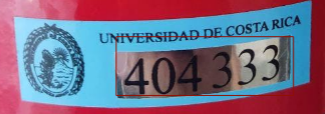
\includegraphics[width=0.5\textwidth]{imagenes/diseño/ejem_placa.PNG}
    \caption{Placa de activo de la Universidad de Costa Rica (ejemplo)}
    \label{ejem_placa}
\end{figure}
\par
La última parte del diseño de la red es el entrenamiento de la misma, por medio de alimentación de datos de entrada. En este caso se utilizó un total de 30 placas capturadas en diferentes activos a través de la facultad de ingeniería y de la EIE. El modelo visto en la Figura \ref{ejem_placa} no es el único existente, sino que se encuentran modelos más antiguos, éstos también fueron considerados dentro del entrenamiento para tener una amplia gama de respuesta por parte de la red. 
\par
Una vez terminado el proceso de entrenamiento se diseñó un código capaz de interactuar con la API de Nanonets, que recibe las imágenes, en este caso en forma de archivo binario, para poder procesarla por medio de la red. La API devuelve una salida con diferentes parámetros escaneados de la imagen en formato JSON, pero únicamente se tomó en cuenta el \lstinline{ocr_text}. La conexión se realizó por medio de el paquete de requests, que permite realizar solicitudes a servidores y servicios API utilizando una llave personal para acceder a ellas (la llave fue provista por Nanonets para la implementación de la aplicación). A continuación se muestran el código de conexión al servidor y para extraer la respuesta respectivamente: 

\begin{lstlisting}[language=Python,frame=single,caption=Código para envío de las placas y recibimiento del texto de la misma (creación propia), inputencoding=latin1]
url = 'https://app.nanonets.com/api/v2/OCR/Model/34353217-1d3f-4511-b86f-e24e842e66e8/LabelFile/?async=false'
data = {'file': open(self.captura_actual, 'rb')}
response = requests.post(url, auth=requests.auth.HTTPBasicAuth('0DeaHQHCf7qAs9n7mFAGmF9gHd6IVMA9', ''), files=data)
\end{lstlisting}

\begin{lstlisting}[language=Python,frame=single,caption=Código para extracción del texto de la placa de la respuesta de la red neuronal (creación propia), inputencoding=latin1]
self.placa_actual = response_json["result"][0]['prediction'][0]['ocr_text']
\end{lstlisting}

\section{Base de datos}
La base de datos se diseñó pensando en que se debía tener un modelo intuitivo que fuese fácil de manipular, donde los datos pudiesen ser exportados de manera sencilla a algún formato conocido por los usuarios. Por ello se utilizó una base de datos relacional, que constará de únicamente una tabla, la cual está definida como la tabla \ref{table1}. 
\begin{table}[H]
\centering
\resizebox{\columnwidth}{!}{\begin{tabular}{cccc}
\hline
Placa (primary key)        & ubicación                    & tipo de activo           & descripción                              \\ \hline
Número de placa del activo & Donde se encuentra el activo & Clasificación del activo & Descripción más detallada de los activos \\ \hline
\end{tabular}}
\caption{Tabla que se implementó en la base de datos}
\label{table1}
\end{table}

\par
Para la creación de la tabla se instaló un servidor local por medio de la herramienta MySQL, que permitió realizar la base de datos de manera local, para realizar las pruebas necesarias dentro del desarrollo de la aplicación. La creación de la tabla dentro de la base de datos se realizó por medio de un script de Python que accediera a la base de datos y generara una solicitud para una tabla nueva con las columnas definidas previamente. El script además dentro de la creación de las columnas define el \textit{Primary Key}, que representa la identificación de cada uno de los registros, no es necesario hacer una asignación automática, puesto que se utilizaría la placa como identificación de cada uno de los registros. El paquete de python utilizado para la gestión de bases de datos fue el nativo de MySQL llamado MySQL Connector, este se instaló dentro del paquete de MYSQL community. El código del script de Python implementado se puede ver a continuación:
\newpage
\begin{lstlisting}[language=Python,frame=single,caption= Script de python para la conexión a una base de datos (creación propia), inputencoding=latin1]
import mysql.connector

db = mysql.connector.connect(
    host='localhost',
    user='root',
    passwd='InventarioEIE2409',
    database='inventarioeie'
)
mycursor = db.cursor()
\end{lstlisting}
\par
Esta sección de código realiza una conexión simple al servidor local de la base de datos, con los credenciales del usuario root para pdoer tener manejo completo de la misma. Dentro de los accesos realizados más adelante no es necesario utilizar una acceso root, puesto que no se estará modificando la tabla y su estructura, sino únicamente añadiendo y modificando datos dentro. Además crea un cursor, el cual es el encargado de realizar todas las operaciones para la creación de bases de datos, tablas y toda la inserción, eliminación y modificación de datos en general, es decir maneja cada una de las solicitudes a la BD. 
\begin{lstlisting}[language=Python,frame=single,caption= Script de python para la creación de una tabla en una base de datos (creación propia), inputencoding=latin1]
mycursor.execute("CREATE TABLE Activos (placa int PRIMARY KEY, ubicacion TEXT(65535), tipo_de_activo TEXT(65535), descripcion TEXT(65535))")
\end{lstlisting}
\par
La anterior sección del script, únicamente creó la tabla nueva llamada \textbf{Activos}, con todos los parámetros necesarios, definiendo así donde se almacenarían los datos a futuro. Los valores que se dieron al tipo de variable de cada una de las columnas es la longitud que puede tener la misma. Para asegurar una generalidad y funcionamiento seguro, se utilizó el valor máximo para cada tipo de variable (65535 caracteres).
\par
Todas y cada una de las funciones que gestionan los accesos y las escrituras a la base de datos se implementaron como funciones dentro del wrapper de la aplicación, ya que es necesario que el funcionamiento se de durante el uso de la aplicación. 




\section{Wrapper de la aplicación}
 El wrapper de la aplicación tiene como funcionamiento crear una capa que permita la conexión de la base de datos y de la red neuronal con el usuario y entre sí. Se utilizó la librería KivyMD, las cual sirve para la creación de interfaces gráficas multiplataforma. Esto permite que el diseño sea utilizable tanto en la plataforma de desarrollo (donde se usó windows), cómo en la plataforma de distribución (android), ya que los elementos que contiene se adaptan a respuestas físicas (como la de un mouse) y a respuestas táctiles (como en dispositivos móviles).
 \par
 KivyMD es una derivación de la librería Kivy, pero que utiliza un diseño moderno (basado en el estilo gráfico de Android actual Material Design 3) para sus elementos. Se realizó de esta forma para que la experiencia de usuario fuese la mejor posible. 
\par
 Inicialmente se construyó el esqueleto de la aplicación, el cual no contiene elementos en el, pero permite inicializar el funcionamiento. KivyMD utiliza programación orientada a objetos para definir a los esqueletos, por lo que se creó la clase \textbf{Inventario}. Esta clase consta de 4 métodos o funciones internas y un constructor. 
 \par
 El constructor se diseñó con diferentes atributos, los obligatorios establecidos por KivyMD, que son: la versión de Material Design que se utilizó (Material Desing 3) y el tema que utiliza la aplicación (esquema de colores). Luego se definió los atributos propios los cuales fueron: La captura actual (string con la dirección de la captura actual), placa actual (string con la placa que se escaneó más recientemente) y el atributo \textit{is registered} (booleano que determina si la placa que se escaneó se encuentra previamente almacenada en la base de datos). El objetivo principal de estas definiciones se basó en la captura de variables de interés que deriven de los métodos de la aplicación.
 \par
 Lo último contenido dentro del constructor, es la pantalla, que importa toda la definición de la interfaz gráfica para mostrarla al usuario. Se escribió las definiciones de la pantalla en la variable \textit{layouts} como un string en lenguaje declarativo de Kivy, que es una forma alternativa, intuitiva y mayormente documentada para el acomodo de los elementos gráficos de la aplicación. En la figura \ref{screen1} se muestra la pantalla principal de la aplicación.
\begin{figure}[H]
    \centering
    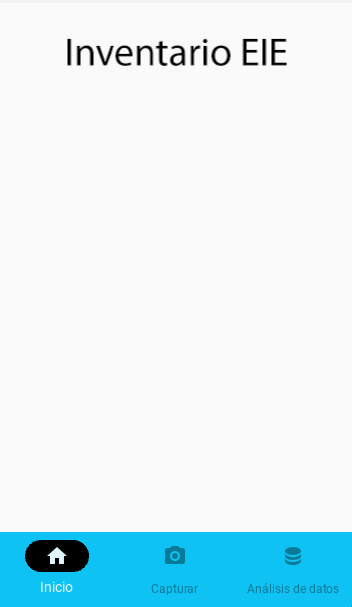
\includegraphics[width=0.35\textwidth]{imagenes/diseño/pantalla1.png}
    \caption{Pantalla principal de la aplicación}
    \label{screen1}
\end{figure}
\par
La forma en la que el lenguaje de Kivy acomoda los elementos de la aplicación es jerárquica, por lo que inicialmente se debió seleccionar el tipo de pantalla deseada, esta usualmente determina como se ve la interfaz general de la aplicación. El nivel principal de la jerarquía que se implementó fue \textit{BottomNavigationLayout}, que contiene una barra inferior con botones para seleccionar la pantalla a la que se accede. Luego en nivel 2 se definió 3 pantallas: inicio, captura y análisis de datos. El nivel 3 siendo el último nivel contiene los elementos dentro de las 3 pantallas del nivel 2.
\par
La pantalla de inicio o pantalla principal, solamente despliega el logo de la aplicación, que se creó a partir de la tipografía de la EIE y un mensaje de bienvenida para los usuarios. 
\par
\begin{figure}[H]
    \centering
    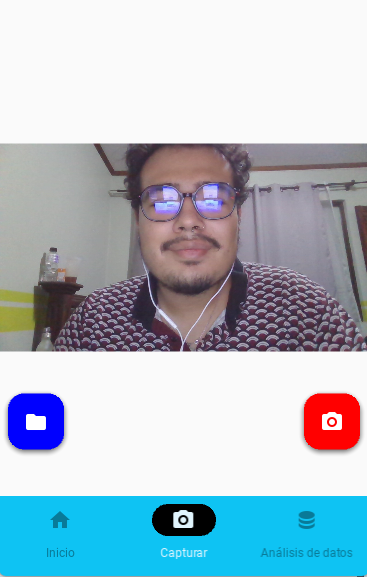
\includegraphics[width=0.35\textwidth]{imagenes/diseño/pantalla2.png}
    \caption{Pantalla de captura de la aplicación}
    \label{screen2}
\end{figure}
\par
La pantalla de captura, que se mostró en la figura \ref{screen2}, contiene 2 elementos: Una imagen en tiempo real de la cámara principal del dispositivo que corre la aplicación y un botón de captura. El botón de captura al ser presionado activa la función \verb|capture(self)|, que almacena en la ubicación actual la imagen de la cámara, asignando un nombre con único y aleatorio, guarda la dirección completa del archivo en \verb|self.captura_actual| y activa la función de \verb|ocr_scan(self)|. En caso de que la imagen se procesó correctamente muestra un mensaje en pantalla para que el usuario avance al análisis de datos y contrariamente un mensaje de error para que el usuario vuelva a tomar la foto.
\par
La función \verb|ocr_scan(self)| implementa tanto el Listing 3.1 cómo el Listing 3.2, si el API de Nanonets devuelve una respuesta con la placa procesada en formato de string retorna un \verb|True|, de lo contrario un \verb|False|, que sirve para activar los mensajes finales en la función de captura.
\par
\begin{figure}[H]
    \centering
    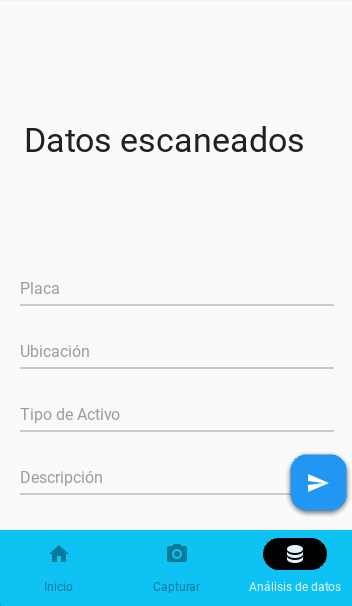
\includegraphics[width=0.35\textwidth]{imagenes/diseño/pantalla3.png}
    \caption{Pantalla de análisis de datos de la aplicación}
    \label{screen3}
\end{figure}
Por último la pantalla de análisis de datos, mostrada en la figura \ref{screen3}, inicialmente al ser presionada activa la función \verb|rev_placa(self)| que se diseñó para verificar la existencia de la placa escaneada dentro de la base de datos. La función inicialmente conecta con el servidor, crea un cursor para ejecutar solicitudes para luego importar todos los datos de la BD. Antes de buscar la placa actual entre todos los datos registrados, pone el valor de \verb|self.is_registered| en falso y si la función logra encontrarla dentro dde la DB, la convierte en verdadero. Cuando \verb|self.is_registered| se encuentra en verdadero, despliega un mensaje en pantalla avisando al usuario de la existencia previa y de la posibilidad de modificar los valores directamente en los campos de texto. Si \verb|self.is_registered| está en falso, se sustituye únicamente el valor de la placa y se despliega un aviso para que el usuario proceda a llenar los datos del activo.
\par
Cuando el usuario decide que ya modificó o agregó los datos del registro, únicamente debe tocar el botón de envío, que activa la función \verb|registrar_placa(self)|. Inicialmente la función conecta con el servidor y crea un cursor, para de forma seguida analizar \verb|self.is_registered|, debido a que los procesos de un registro nuevo y la modificación de un registro son distintos. Cuando el atributo es verdadero se utilizó el siguiente código:
\newpage
\begin{lstlisting}[language=Python,frame=single,caption= Modificación de registro previamente existente (creación propia), inputencoding=latin1]
mycursor.execute("UPDATE Activos SET ubicacion = %s, tipo_de_activo = %s, descripcion = %s WHERE placa = %s", (self.root.ids.ubicacion.text, self.root.ids.active_type.text, self.root.ids.descrip.text, self.placa_actual))
            db.commit()
            toast("Placa actualizada!")
\end{lstlisting}
\par
Los parámetros dentro del \verb|execute|, corresponden a los strings contenidos en las cajas de texto de la pantalla de análisis de datos. Cuando no se encuentra el valor registrado en la BD, el código que se usó fue el siguiente:
\begin{lstlisting}[language=Python,frame=single,caption= Registro nuevo de activo (creación propia), inputencoding=latin1]
mycursor.execute("INSERT INTO Activos (placa, ubicacion, tipo_de_activo, descripcion) VALUES (%s, %s, %s, %s)", (self.placa_actual, self.root.ids.ubicacion.text, self.root.ids.active_type.text, self.root.ids.descrip.text))
            db.commit()
            toast("Placa registrada!")
\end{lstlisting}
\par
De esta forma se definió el wrapper y sus elementos, que implementan los otro módulos del diseño inicial, afirmando así la base que se mostró en la figura \ref{appdiagram}. 







% --------------------------------
\chapter{Análisis de resultados}
% --------------------------------
\label{C:sobre_LaTeX}
En esta sección se comprobó el funcionamiento completo de la aplicación diseñada por medio de un estudio de caso, en el que se tomó la placa de un activo para poder realizar el proceso completo de registro. A partir de ello se discutió los resultados obtenidos y se mostró cuales posibles escenarios alternativos podría presentar en su funcionamiento.
\par

\section{Estudio de caso}
Para este estudio de caso se tomó la placa de una silla de la sala de estudio (que previamente se registró en las pruebas), una placa de un monitor sin registrar y una foto sin ninguna placa en ella. Se inició colocando la placa de la silla de la sala de estudio dentro del rango de la cámara, cómo se puede apreciar en la figura \ref{r:uno}. Este es el primer paso necesario para el registro, es importante destacar, que debido al proceso de entrenamiento que se aplicó a la red neuronal y a los parámetros de preprocesado de imágenes utilizado, los resultados pueden ser obtenidos aún cuando la imagen no sea lo más clara o no esté lo suficientemente centrada. 

\begin{figure}[ht]
    \centering
    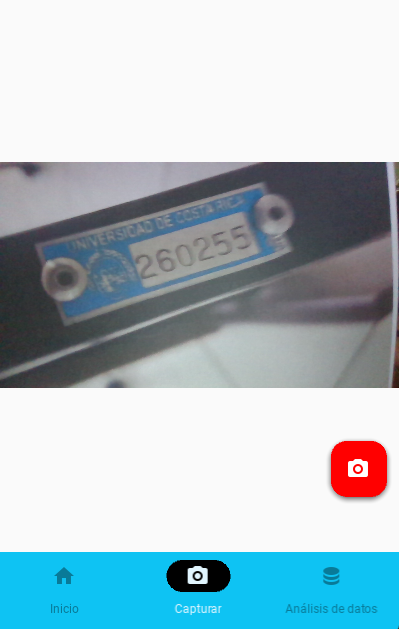
\includegraphics[width=0.35\textwidth]{imagenes/resultados/uno.png}
    \caption{Paso uno del registro de placas}
    \label{r:uno}
\end{figure}
\par
Una vez que se determinó que la imagen se encontraba apta para que la red la procese, se oprime el botón rojo de captura, lo cual en caso de ser correcto muestra una notificación en pantalla como se puede observar en la figura \ref{r:dos}, por lo que el usuario se notifica de la posibilidad de avanzar al análisis de datos.
\begin{figure}[ht]
    \centering
    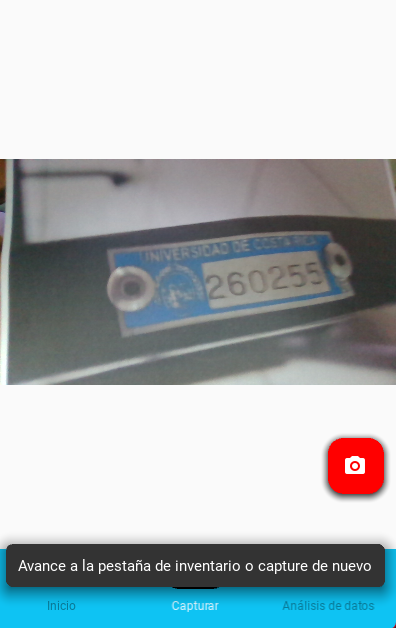
\includegraphics[width=0.35\textwidth]{imagenes/resultados/dos.png}
    \caption{Paso dos del registro de placas}
    \label{r:dos}
\end{figure}
\par
Cuando se oprime el botón de análisis de datos, se accede a la BD y se despliega la información de la placa, en este caso se escaneó una placa previamente registrada, por lo que los datos anteriores también se presentan en el espacio lleno para que se puedan ver y modificar, así como se ve en la figura \ref{r:tres}.
\begin{figure}[ht]
    \centering
    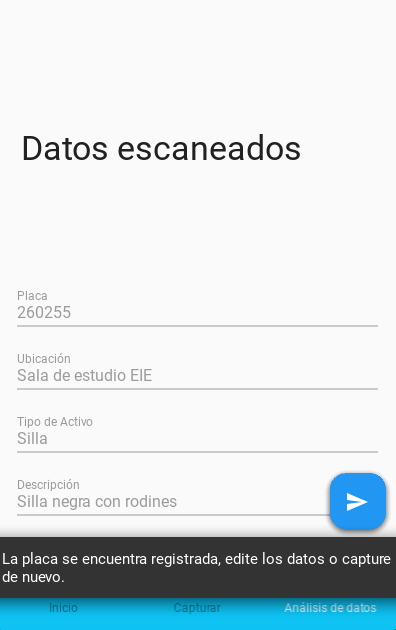
\includegraphics[width=0.35\textwidth]{imagenes/resultados/tres.png}
    \caption{Paso tres del registro de placas}
    \label{r:tres}
\end{figure}
\par
El usuario deberá modificar los valores que así lo requieran y una vez se decide que la información está completa, únicamente se oprime el botón de enviar y cuando se completa la solicitud a la BD, la aplicación despliega un mensaje como en la figura \ref{r:cuatro}. Con esto se completa un proceso de registro (en este caso modificación) de un activo de la EIE. 
\begin{figure}[ht]
    \centering
    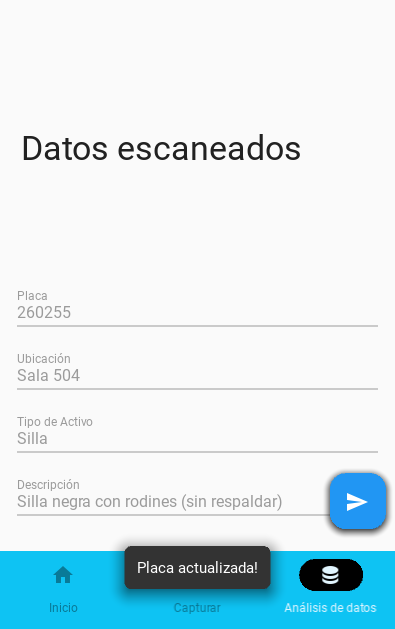
\includegraphics[width=0.35\textwidth]{imagenes/resultados/cuatro.png}
    \caption{Último paso del registro de placas}
    \label{r:cuatro}
\end{figure}
\par
El registro puede presentar variaciones dependiendo de lo que se requiere hacer, cuando una placa no se encuentra en la base de datos, únicamente el espacio de placa se llena por el usuario para que pueda añadir los valores de la misma como en la figura \ref{r:cinco}. Una vez registrada el mensaje que despliega la aplicación al usuario es la de registro exitoso en vez de que se actualizó la placa. Otro caso es cuando la imagen es ilegible por la red neuronal, aquí se avisa al usuario desde la misma pantalla de captura, que no es posible identificar la placa y que debe retomar la captura, de forma equivalente a la figura \ref{r:seis}.
\begin{figure}[ht]
    \centering
    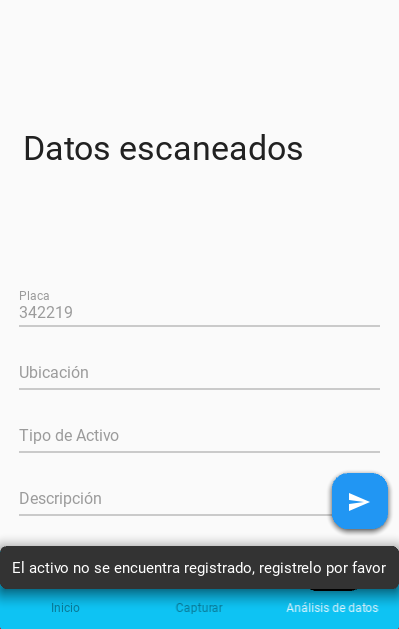
\includegraphics[width=0.35\textwidth]{imagenes/resultados/cinco.png}
    \caption{Comportamiento de la aplicación ante un registro de una nueva placa.}
    \label{r:cinco}
\end{figure}
\begin{figure}[ht]
    \centering
    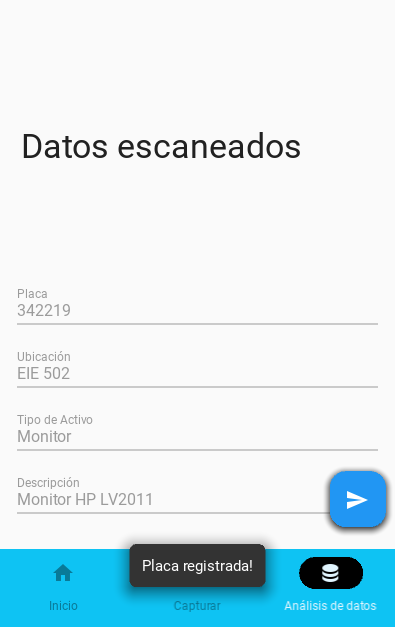
\includegraphics[width=0.35\textwidth]{imagenes/resultados/seis.png}
    \caption{Comportamiento de la aplicación ante una captura ilegible para la red neuronal.}
    \label{r:seis}
\end{figure}
% ----------------------------------------
  \chapter{Conclusiones y recomendaciones}
% ----------------------------------------
\label{C:conclusiones}
\section{Conclusiones}
\begin{itemize}
    \item Se logró crear, entrenar y utilizar una red neuronal capaz de procesar texto por medio de OCR para el procesamiento de las placas de la EIE.
    \item Se creó correctamente una base de datos relacional, que posee una tabla con los campos necesarios para registrar los datos más relevantes del inventariado solicitado por la Universidad de Costa Rica a cada unidad académica.
    \item Se implementó una aplicación con interfaz gráfica intuitiva, que permite a los usuarios registrar activos de forma sencilla y gráfica.
    \item Se sentó una base para la compilación de la aplicación en plataformas Android que toma en cuenta las diferencias para el entorno dentro del diseño.
    \item Se comprobó el funcionamiento integral de la aplicación y su funcionamiento óptimo para diferentes escenarios y posibles errores humanos en el uso de la misma.

    
\end{itemize}


\section{Recomendaciones}
\begin{itemize}
    \item Utilizar contenido educativo de personas que hayan realizado alguna función necesaria previamente como forma de aclaración de la documentación oficial
    \item Delimitar los proyectos de forma más especifica para el tiempo dado durante el curso de Proyecto Eléctrico.
    \item Diseñar los programas por medio de bloques que finalmente funcionen en conjunto, para facilitar el proceso de corrección de errores y de un único diseño extenso.
    \item Utilizar un sistema de control de versiones (cómo git) para poder monitorear el proceso y regresar a versiones previamente desarrolladas que pudisen contener código necesario para una versión más reciente.
\end{itemize}

% 8. APÉNDICES
\appendix
\input{apendices/A_ejemplo.tex}




\backmatter

% 9. BILIOGRAFÍA
\bibliographystyle{plain}
\bibliography{bibliografia/bibliografia.bib}

%%%%%%%%%%%%%%%%%%%
\end{document}
%%%%%%%%%%%%%%%%%%%

% ----------------------------------------------
% Plantilla elaborada por Fabián Abarca Calderón
% ----------------------------------------------